\section{Training}
\label{sec:training}
This chapter is giving an introduction into the training and how the training was done. For each configuration a plot with three rows is represented. First row is showing the disriminator and generator loss. The following three are metrics, which approximate the performance of the training and give insights into the ability of creating undistinguishing data. The precison and recall from the best training iteration is shown later or in the appendix.

\begin{figure}[htbp]
    \centering
    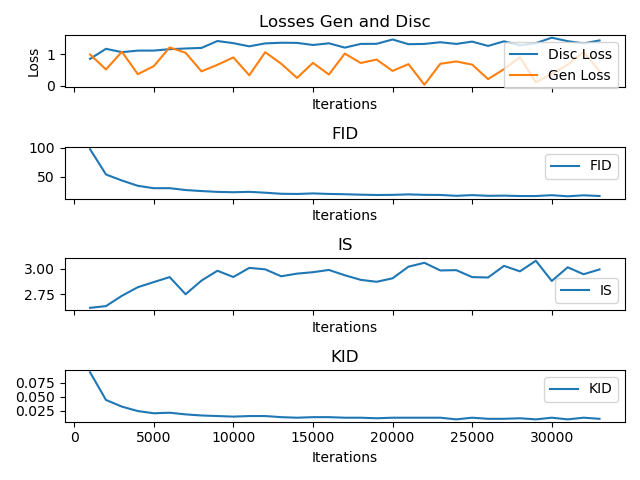
\includegraphics[width=0.8\textwidth]{training/loss_resnet_sn_fm.png}
    \caption{Resnet specral normalization and feature matching}
    \label{fig:training_resnet_sn_fm}
\end{figure}

\begin{figure}[htbp]
    \centering
    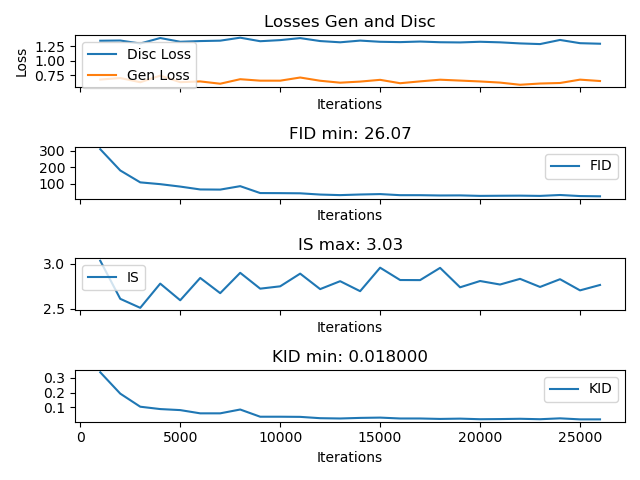
\includegraphics[width=0.8\textwidth]{training/loss_dcgan_only.png}
    \caption{classical DCGAN}
    \label{fig:training_scgan}
\end{figure}


\begin{figure}[htbp]
    \centering
    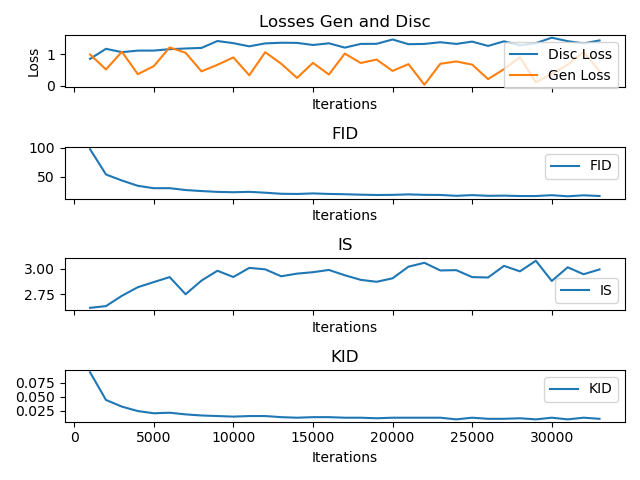
\includegraphics[width=0.8\textwidth]{training/loss_resnet_sn_hinge.png}
    \caption{Resnet specral normalization and hinge}
    \label{fig:training_resnet_sn_hinge}
\end{figure}